%% LyX 2.1.3 created this file.  For more info, see http://www.lyx.org/.
\documentclass[a4paper,english,12pt]{article}
\usepackage{%
	amsmath,%
	amsfonts,%
	amssymb,%
	amsthm,%
	hyperref,%
	url,%
	latexsym,%
	epsfig,%
	graphicx,%
	psfrag,%
	subfigure,%	
	color,%
	tikz,%
	pgf,%
	pgfplots,%
	pgfplotstable,%
	pgfpages,%
	proofs%
}

\usepgflibrary{shapes}
\usetikzlibrary{%
  arrows,%
	backgrounds,%
	chains,%
	decorations.pathmorphing,% /pgf/decoration/random steps | erste Graphik
	decorations.text,%
	matrix,%
  positioning,% wg. " of "
  fit,%
	patterns,%
  petri,%
	plotmarks,%
  scopes,%
	shadows,%
  shapes.misc,% wg. rounded rectangle
  shapes.arrows,%
	shapes.callouts,%
  shapes%
}

\theoremstyle{plain}
\newtheorem{thm}{Theorem}[section]
\newtheorem{lem}[thm]{Lemma}
\newtheorem{prop}[thm]{Proposition}
\newtheorem{cor}[thm]{Corollary}

\theoremstyle{definition}
\newtheorem{defn}[thm]{Definition}
\newtheorem{conj}[thm]{Conjecture}
\newtheorem{exmp}[thm]{Example}
\newtheorem{assum}[thm]{Assumptions}

%\theoremstyle{remark}
\newtheorem{rem}{Remark}
\newtheorem{note}{Note}

\makeatletter
\def\th@plain{%
  \thm@notefont{}% same as heading font
  \itshape % body font
}
\def\th@definition{%
  \thm@notefont{}% same as heading font
  \normalfont % body font
}
\makeatother
\date{}
%\usepackage[T1]{fontenc}
%\PassOptionsToPackage{normalem}{ulem}
%\usepackage{ulem}
%\usepackage{caption}
%\makeatletter
%\usepackage{multicol}
%%%%%%%%%%%%%%%%%%%%%%%%%%%%%% LyX specific LaTeX commands.
%\pdfpageheight\paperheight
%\pdfpagewidth\paperwidth


%\makeatother

%\usepackage{babel}
\begin{document}

\title{Lecture 5: Image, Inverse Image, Composition and Inverse of Functions}
\author{Parimal Parag}
\maketitle

\section{Image and Inverse Image}
Let $A$ and $B$ be sets and $f:A\rightarrow B$ be a function. 
\begin{defn}[Image] For every $P\subseteq A$, the \textbf{image} of $P$ under $f$ is defined as follows:
\begin{equation*}
f_*(P)  =\{b\in B: b=f(p) \textnormal{ for some } p\in P\} =\{f(p):p\in P\}
\end{equation*}
\end{defn}

\begin{defn}[Inverse Image] For every $Q\subseteq B$, the \textbf{inverse image} (or \textbf{preimage}) of $Q$ under $f$ is defined as follows:
\begin{equation*}
f^*(Q)  =\{a\in A: f(a)=q \textnormal{ for some } q\in Q\} =\{a\in A:f(a)\in Q\}
\end{equation*}
\end{defn}

\begin{figure}[h]
\centering
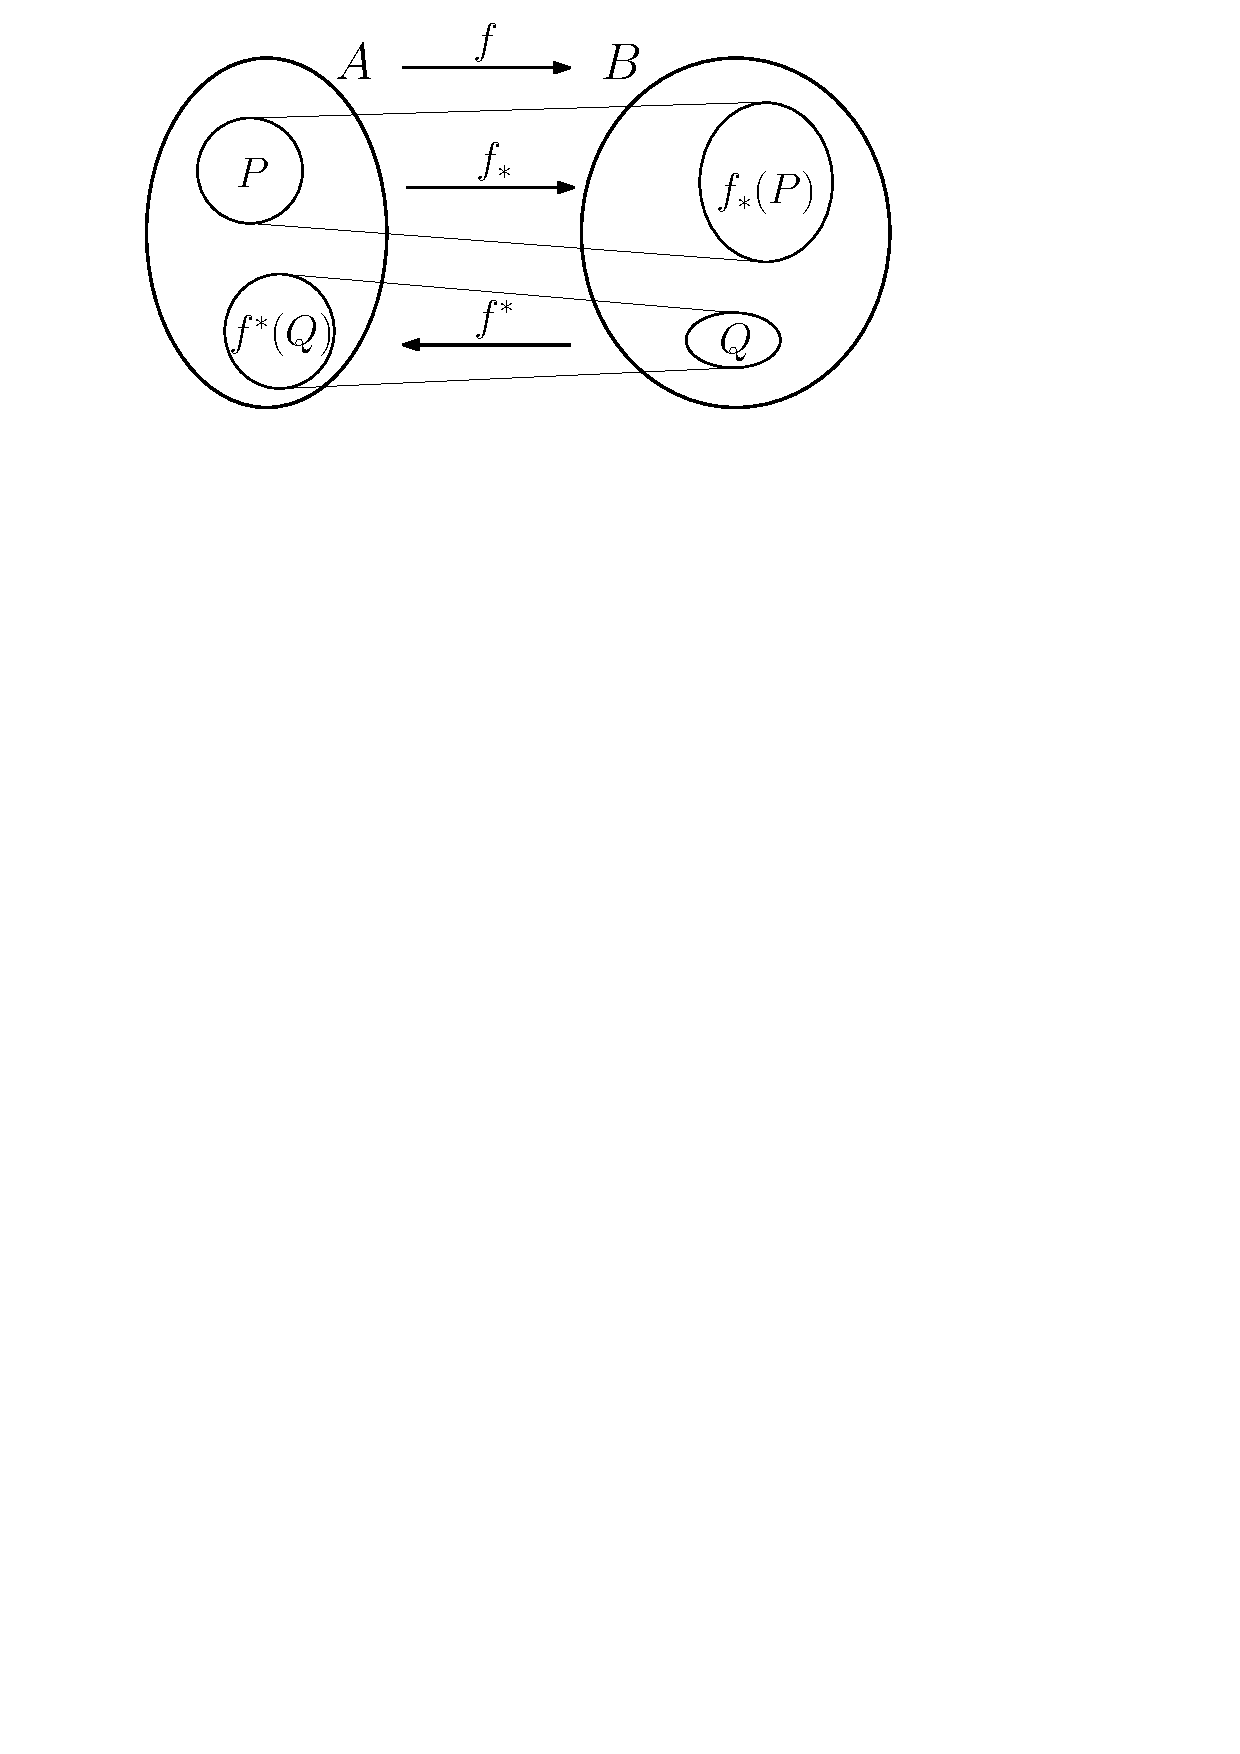
\includegraphics[scale=0.6]{Figures/l5f1_img-invimg.pdf}
\caption{}
\end{figure}

\textbf{Remarks:}
\begin{enumerate}[i)]
\item For every $P\subseteq A$, $\emptyset \neq f_*(P)\subseteq B$ and $|P|\geqslant |f_*(P)|$. The \textbf{range} (or \textbf{image}) of $f$ is the set $f_*(A)$. The range need not be equal to the codomain.
\item For every $Q\subseteq B$, $f^*(Q)\subseteq A$, possibly be empty, and $|Q|\leqslant |f^*(Q)|$. 
\item Given a function $f:A\rightarrow B$, the process of taking image (inverse image) of subsets of $A$ ($B$) can be thought of as operation of a new function $f_*:2^A\rightarrow 2^B$ ($f^*:2^B\rightarrow 2^A$) on subsets of $A$ ($B$) and induced by $f$.
\item Abuse of notation: 
\begin{enumerate}[a)]
\item Even though $f$ maps elements of $A$ to elements of $B$ and not subsets of $A$ (say $P$) to subsets of $B$ (say $Q$), often $f_*$ is replaced with $f$ for convenience, \textit{i.e.}, $f(P)$ is substituted for $f_*(P)$.
\item Similarly, $f^*$ is replaced with $f^{-1}$ for inverse image. Later, we will look at the \textbf{inverse} of a function $f:A\rightarrow B$ (if it exists) and denote it by $f^{-1}:B\rightarrow A$. If the inverse function of $f$ does not exist, then $f^{-1}(Q)$ is used to refer to the inverse image $f^*(Q)$ of $Q$ under $f$. If the inverse of $f$ exists, then it takes elements and not subsets of $B$ as the argument; and $f^*(Q)=f^{-1}(Q)=f^{-1}_*(Q)$, \textit{i.e.}, $f^{-1}(Q)$ can be used to refer to both the inverse image of $Q$ under $f$ ($f^*(Q)$) and the image of $Q$ under $f^{-1}$ ($f^{-1}_*(Q)$).
\end{enumerate}
\end{enumerate}

\begin{exmp}
Consider the function $f:\mathbb{R}\rightarrow \mathbb{R}$ plotted in Fig.~\ref{func_ex}.\begin{enumerate}[i)]
\item The range of $f$, $f_*(\mathbb{R})=[-3,\infty)\subset \mathbb{R}$.
\item For $P_1=[1.5,1.9]$ and $P_2=[-4.5,-3.3]$, $f_*(P_1)=[1.7,2.5]$ and $f_*(P_2)=[-3,-1]$.
\begin{figure}[h]
\centering
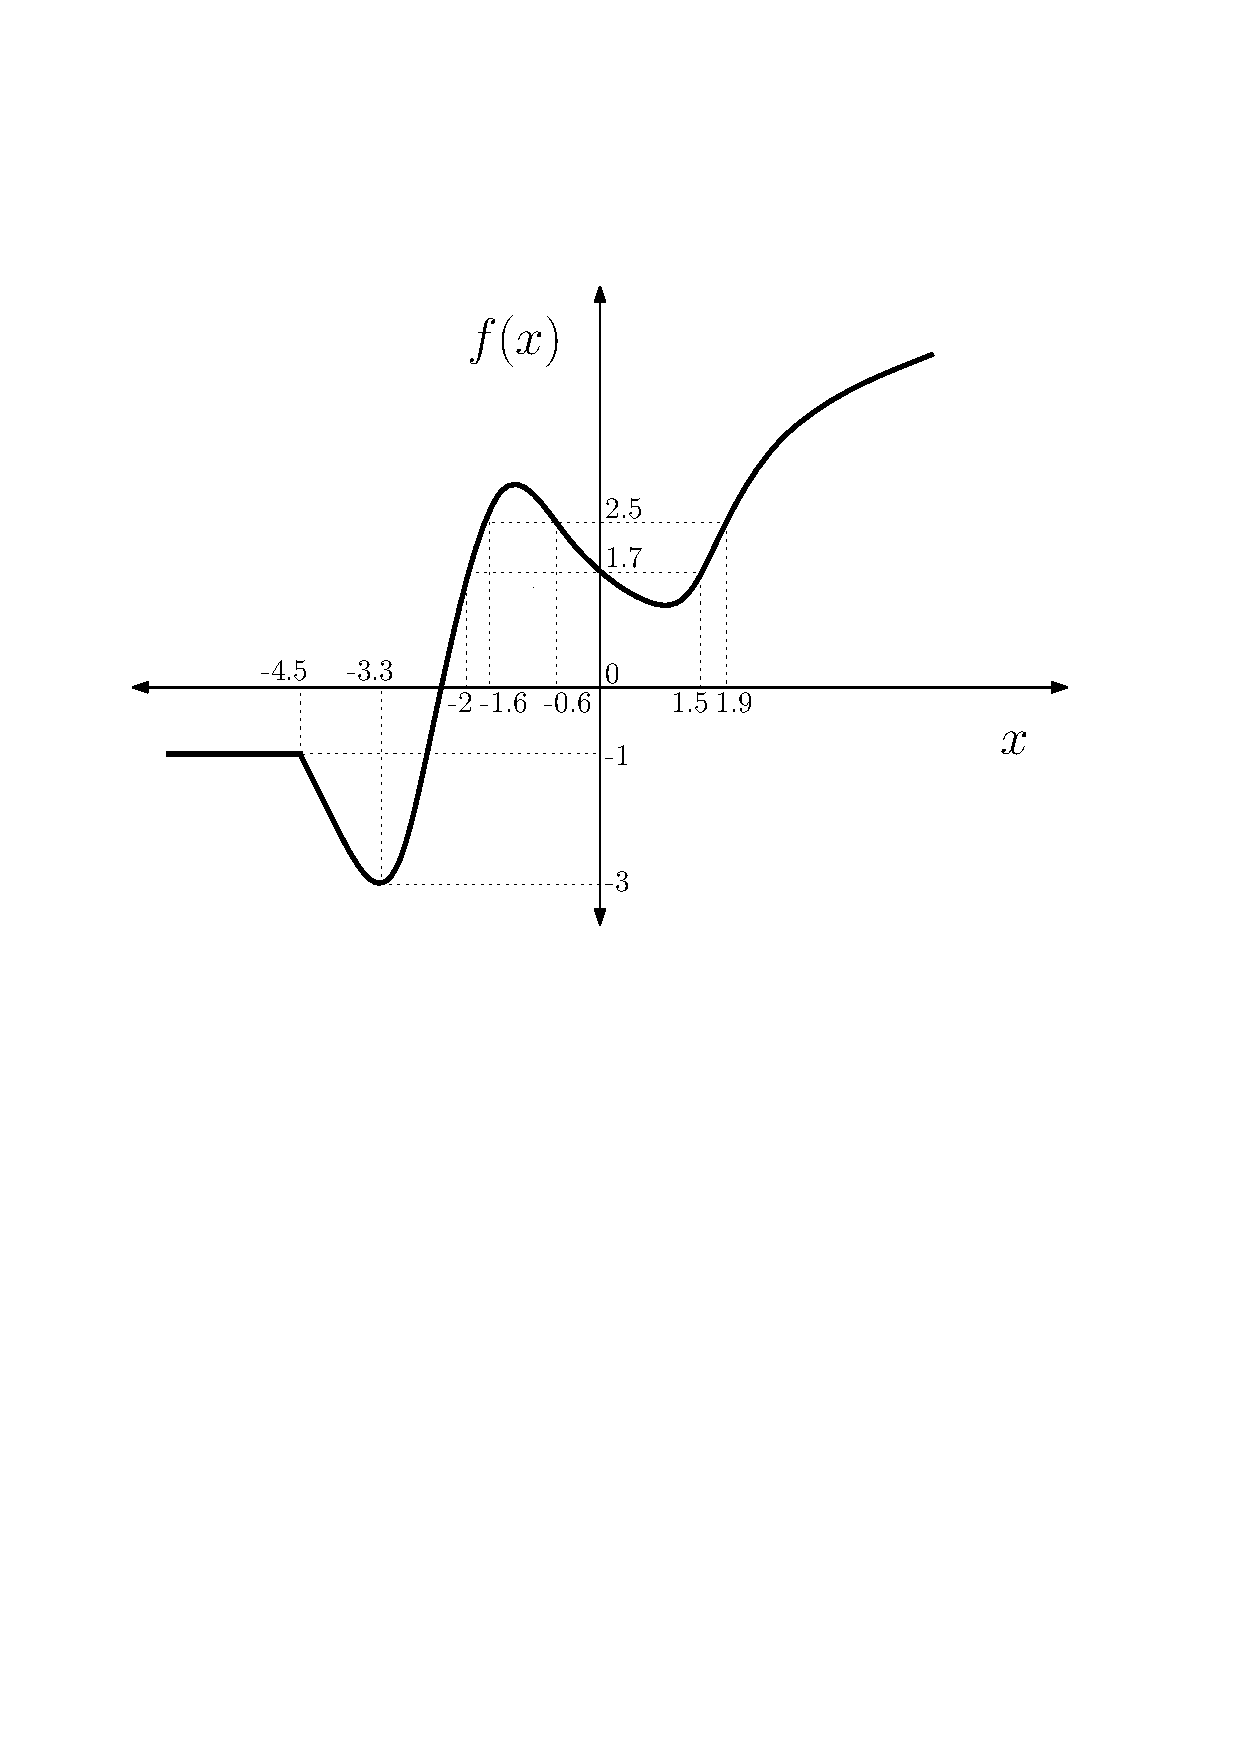
\includegraphics[scale=0.6]{Figures/l5f2_graph.pdf}
\caption{}
\label{func_ex}
\end{figure}
\item For $Q_1=[1.7,2.5]$ and $Q_2=[-4,-3.2]$, $f^*(Q_1)= [-2,-1.6] \cup [-0.6,0] \cup [1.7,2.5]$ and $f^*(Q_2)=\emptyset$.
\item From (i) and (ii), we have that $f^*(f_*(P_1))\neq P_1$, $f^*(f_*(P_2))=P_2$, $f_*(f^*(Q_1))=Q_1$ and $f_*(f^*(Q_2))=Q_2$ (cf. Thrm.~\ref{img-preimg_props}).
\end{enumerate}
\end{exmp}

\begin{thm} Let $A$ and $B$ be sets, let $C,D\subseteq A$ and $S,T\subseteq B$ be subsets, and let $f:A\rightarrow B$ be a function. Let $I,J\neq\emptyset$, let $\{U_i:i\in I\}$ and $\{V_j:j\in J\}$ be indexed families of sets, where $U_i\subseteq A, \forall i\in I$ and $V_j\subseteq B, \forall j\in J$.
\begin{multicols}{2}
\begin{enumerate}[i)]
\item $f_*(\emptyset)=\emptyset$ and $f^*(\emptyset)=\emptyset$.
\item $f^*(B)=A$.
\item $f_*(C)\subseteq S$ iff $C\subseteq f^*(S)$.
\item If $C\subseteq C$ then $f_*(C)\subseteq f_*(D)$.
\item If $S\subseteq T$ then $f^*(S)\subseteq f^*(T)$.
\item $f_*(\bigcup_{i\in I}U_i)=\bigcup_{i\in I}f_*(U_i)$.
\item $f_*(\bigcap_{i\in I}U_i)\subseteq \bigcap_{i\in I}f_*(U_i)$.
\item $f^*(\bigcup_{j\in J}V_j)=\bigcup_{j\in J}f^*(V_j)$.
\item $f^*(\bigcap_{j\in J}V_j)=\bigcap_{j\in J}f^*(V_j)$.
\end{enumerate} 
\end{multicols}
\label{img-preimg_props}
\end{thm}
\noindent (\textit{Hint: Let $X$ and $Y$ be sets. To show $X=Y$, show that $X\subseteq Y$ and $Y\subseteq X$.})

\section{Composition}
\begin{defn}[Composition of Functions] Let $A$, $B$ and $C$ be sets, and let $f:A\rightarrow B$ and $g:B\rightarrow C$ be functions. The \textbf{composition} of $f$ and $g$ is the function $g\circ f:A\rightarrow C$ and is defined as follows:
\begin{equation*}
(g\circ f) (a)  =g(f(a))
\end{equation*}
for all $a\in A$
\end{defn}

\textbf{Remarks:}
\begin{enumerate}[i)]
\item Composition of three or more functions can be defined similarly.
\item Though read/written left to write, while obtaining value of $(g\circ f)(a),a\in A$, $f(a)$ is computed first followed by $g(f(a))$.
\item Function compositions can be visualized by \textit{commutative diagrams}. Following is the commutative diagram for $g\circ f$.
\begin{figure*}[h]
\centering
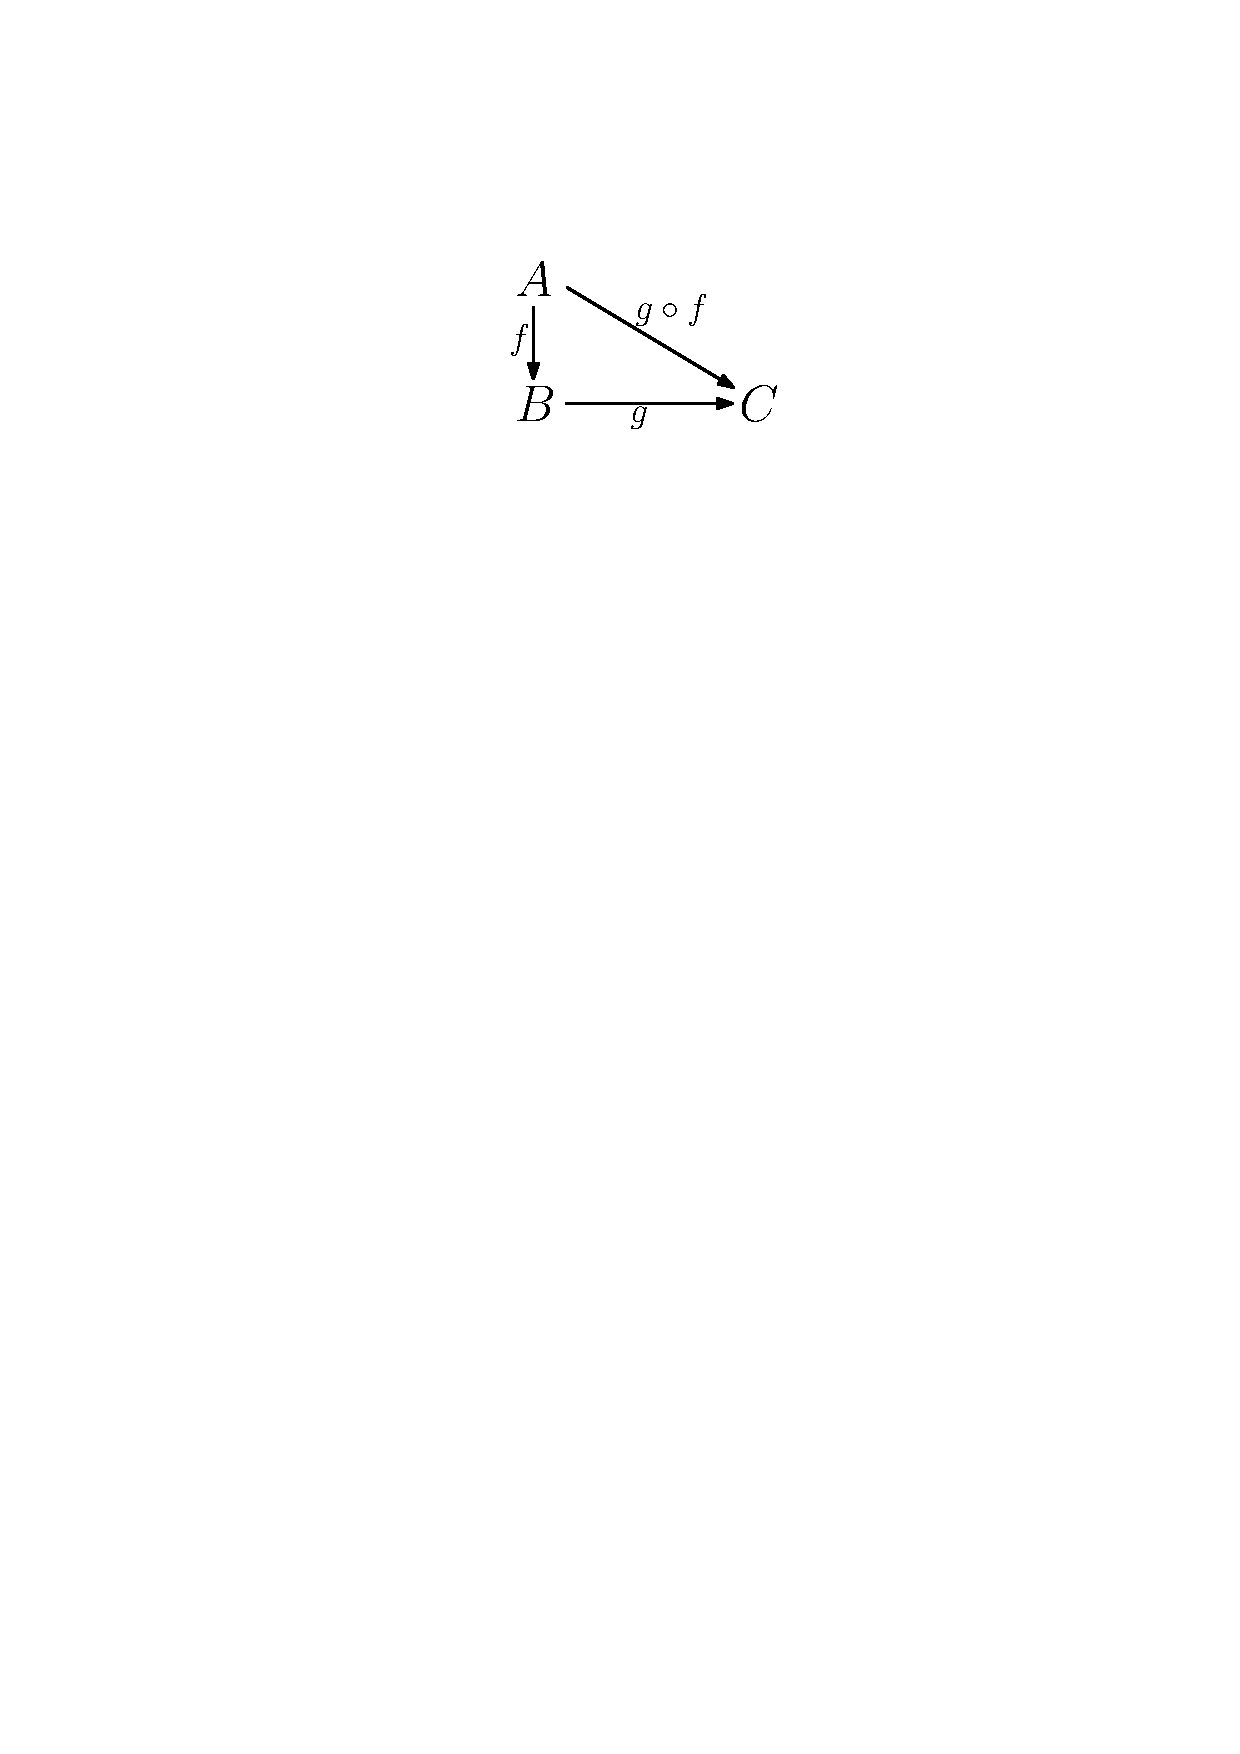
\includegraphics[scale=0.8]{Figures/l5f3_commdiag.pdf}
\end{figure*}
\item If the codomain of the first function ($f$) is equal to the domain of the second ($g$), then the composition $g\circ f$ is defined. (The composition is defined iff the range of the first function is a subset of the domain of the second).
\item If $A=C$, then $f\circ g$ is also defined but need not necessarily be equal to $g\circ f$ or $1_A$.
\item The range of $g\circ f$ is a subset of range of $g$, \textit{i.e.}, $(g\circ f)_*\subseteq g_*$.
\end{enumerate}

\begin{exmp}
Let $f:\mathbb{R}\rightarrow \mathbb{R}$ be defined by $f(x)=x^3$ , $g:[0,\infty)\rightarrow \mathbb{R}$ be defined by $g(x)=\sqrt{x}$ and $h:\mathbb{R}\rightarrow \mathbb{R}$ be defined by $h(x)=2x$. Then 
\begin{enumerate}[i)]
\item $f\circ f:\mathbb{R}\rightarrow \mathbb{R}$ and $(f\circ f)(x)=(x^3)^3$.
\item $(f\circ g):[0,\infty)\rightarrow \mathbb{R}$ and $(f\circ g)(x)=\sqrt{x^3}$.
\item $(f\circ h):\mathbb{R}\rightarrow \mathbb{R}$ and $(f\circ h)(x)=(2x)^3$.
\item $(h\circ f):\mathbb{R}\rightarrow \mathbb{R}$ and $(h\circ f)(x)=2x^3$. (Note that $(h\circ f)\neq (f\circ h)$)
\item $(h\circ g):[0,\infty)\rightarrow \mathbb{R}$ and $(h\circ g)(x)=2\sqrt{x}$.
\item $f\circ h\circ g:[0,\infty)\rightarrow \mathbb{R}$ and $(f\circ h\circ g)(x)=(2\sqrt{x})^3$.
\item $f\circ f\circ h:\mathbb{R}\rightarrow \mathbb{R}$ and $(f\circ f\circ h)(x)=((2x)^3)^3$.
\item $(g\circ g),\,(g\circ f),\,(g\circ h),\,(f\circ g\circ h),\,(g\circ h\circ f),\,(g\circ f\circ h),\,(h\circ g\circ f)$ are not defined.
\end{enumerate}
Similarly, many more functions can be obtained.
\label{ex_comp}
\end{exmp}

\begin{defn}[Coordinate Function] Let $A,A_1,A_2,\ldots,A_n$ be sets for some $n\in \mathbb{N}$ and let $f:A\rightarrow A_1\times A_2\times \ldots \times A_n$ be a function. For each $i\in \{1,2,\ldots ,n\}$, let $f_i:A\rightarrow A_i$ be defined by $f_i=\Pi _i\circ f$, where $\Pi _i:A_1\times A_2\times \ldots \times A_n \rightarrow A$ is the $i^{th}$ projection map. Then, $f_1,f_2,\ldots ,f_n$ are the \textbf{coordinate functions} of $f$.
\end{defn}
Coordinates functions can be represented using a commutative diagram; given below is the commutative diagram for $n=2$.
\begin{figure*}[h]
\centering
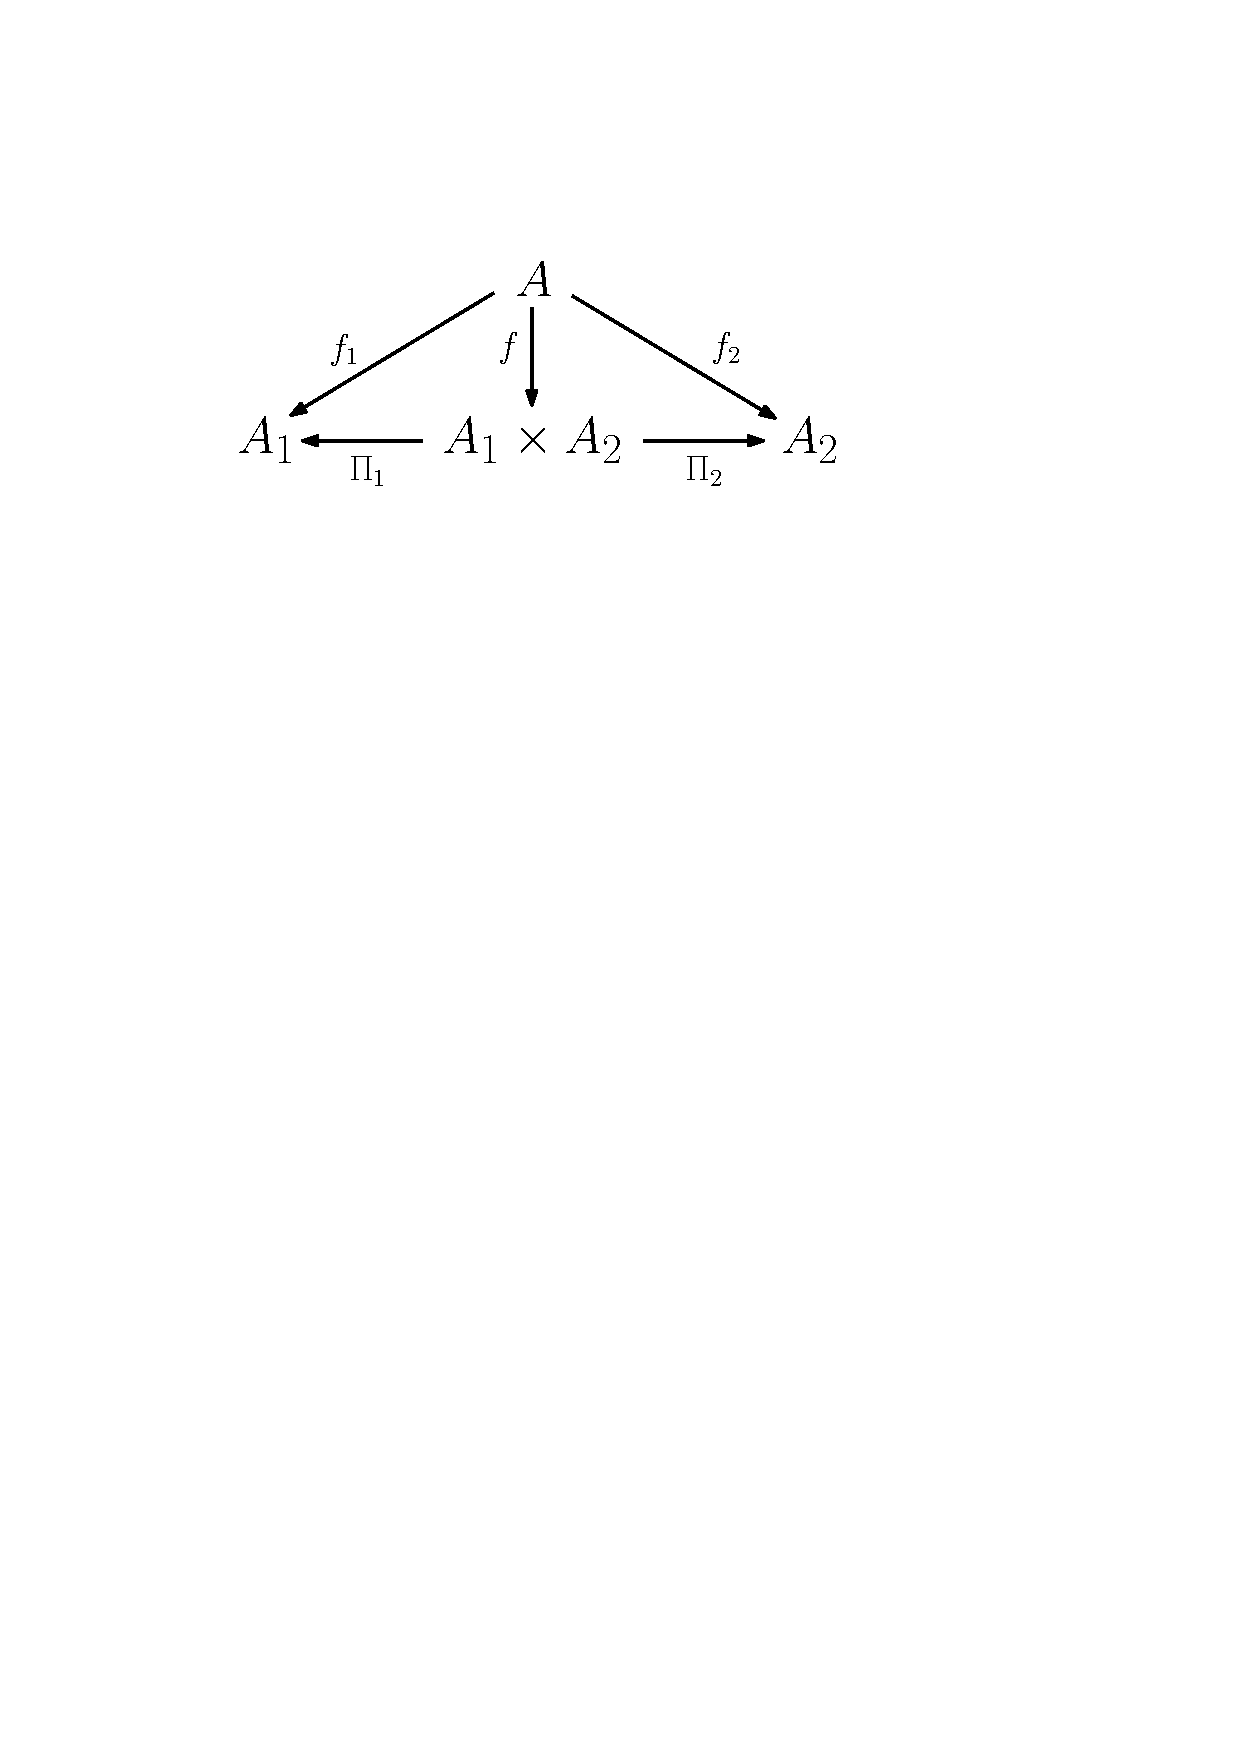
\includegraphics[scale=0.56]{Figures/l5f4_coord.pdf}
\end{figure*}

\begin{exmp}
The function $f:\mathbb{R}^2\rightarrow \mathbb{R}^3$ defined by $f(x,y)=(xy,\,sin(x^2),\,x+y^3)$ has 3 coordinate functions $f_1,f_2,f_3:\mathbb{R}^2\rightarrow \mathbb{R}$ given by 
\begin{equation*}
f_1((x,y))=xy \qquad f_2((x,y))=sin(x^2) \qquad f_3((x,y))=x+y^3
\end{equation*}
\end{exmp}

\begin{lem}
Let $A,\,B,\,C,\,D$ be sets and $f:\rightarrow B,\, g:B\rightarrow C$ and $h:C\rightarrow D$ be functions. Then
\begin{enumerate}[i)]
\item $(h\circ g)\circ f=h\circ (g\circ f)$ \qquad (Associative law)
\item $f\circ 1_A=f$ and $1_B\circ f=f$ \qquad (Identity law)
\end{enumerate}
\end{lem}

\noindent Commutativity does not always hold for function composition (cf. Ex.~\ref{ex_comp}(iv)).

\section{Inverse Function}
\begin{defn}
Let $A$ and $B$ be sets and let $f:A\rightarrow  B$ and $g:B\rightarrow  A$ be functions. Then the function $g$ is 
\begin{enumerate}[i)]
\item a \textbf{right inverse} for $f$ if $f\circ g=1_B$,
\item a \textbf{left inverse} for $f$ if $g\circ f=1_A$ and
\item an \textbf{inverse} for $f$ if it is both a right and left inverse.
\end{enumerate}
\end{defn}
\noindent If $g$ is a left (right) inverse for $f$, then $f$ is a right (left) inverse for $g$.

\begin{exmp}
Let $P$ be the set of all people and $W$ be the set of women with at least one child, and let $c:P\rightarrow W$ be the function that maps a person to their mother and $m:W\rightarrow P$ be the function that maps a woman to her eldest child. 

Choose a person $p\in P$ who is not the eldest of their siblings, and let the eldest sibling of the chosen person be $p'$. Then, $c(p)=w$, for some $w\in W$ and $m(w)=p'\neq p$. Thus, $(m\circ c)(p)\neq p, \forall p\in P$.

Choose a woman $w\in W$. Then, $m(w)=p$ for some $p\in P$ and $c(p)=w$. Thus, $(c\circ m)(w)=w$.

Hence, $m$ has a left inverse ($c$) but no right inverse and $c$ has a right inverse ($m$) but no left inverse.

Had $P$ been the set of people who are eldest of their siblings, then the maps $c$ and $m$ would have been inverse of each other.

Had $m$ been a map from $P$ to $P$, then neither right nor left inverse of either maps would not have existed.
\end{exmp}

\begin{lem}
Let $A$ and $B$ be sets, and let $f:A\rightarrow B$ be a function.
\begin{enumerate}[i)]
\item If $f$ has an inverse, then it is unique.
\item If $f$ has a right inverse $g$ and a left inverse $h$, then $g=h$, and hence $f$ has an inverse.
\item If $f$ has an inverse $g$, then $g$ has an inverse, which is $f$.
\end{enumerate}
\end{lem}

\begin{defn}
Let $A$ and $B$ be sets, and let $f:A\rightarrow B$ be a function. If $f$ has an inverse, then the inverse is denoted by $f^{-1}:B\rightarrow A$.
\end{defn}

\noindent \textbf{Remarks:} 
\begin{enumerate}
\item $f^{-1}\circ f=1_A$ and $(f^{-1}\circ f)(a)=a,\,\forall a\in A$.
\item $f\circ f^{-1}=1_B$ and $(f\circ f^{-1})(b)=b,\,\forall b\in B$.
\item Given the graph of a function $f:A\rightarrow B$, where $A,B\subseteq \mathbb{R}$, the inverse function $f^{-1}$ can be plotted by reflecting the graph of $f$ in the line $x=y$. This is same as first reflecting $f$ in \textit{y-axis} followed by $90^{\circ}$ clockwise rotation.
\end{enumerate}


\end{document}
